%%%%%%%%%%%%%%%%%%%%%%%%%%%%%%%%%%%%%%%%%%%%%%%%%%%
% multithreading.tex
%%%%%%%%%%%%%%%%%%%%%%%%%%%%%%%%%%%%%%%%%%%%%%%%%%%
\label{sec:multithreading}

\subsection{\textbf{The transition to multithreading}}
The emergence of multi-core and many-core processors has been a well-established
trend in the chip-making industry during the past decade.  While this paradigm 
guarantees the continued increase of CPU performance, it requires some 
adaptation of existing code in order to better utilize these architectures.  In
typical \Gfour{} simulations the most widespread approach for exploiting 
parallelism is job or process parallelism.  This is the spawning of multiple 
copies of the same process, and is being used in large-scale production by HEP 
experiments to exploit today's hardware.  However a key challenge for this 
approach is that the amount of random access memory (RAM) required scales 
linearly with the number of processes.  As the number of cores increases beyond
8 or 16, the amount of RAM may become a limiting factor unless a robust solution
for the sharing of memory between processes (or an alternative method) can be 
adopted in production systems.

This is especially true for co-processor technologies in which a high core count
is associated with a relatively limited amount of RAM, as in the Intel Xeon Phi 
co-processor card model 7120P, which hosts 16GB of RAM for 61 physical cores.

In \Gfour{} an alternative solution was developed, in which multithreaded 
applications share a substantial part of their data between threads in order to
significantly reduce the memory footprint.  In this design the memory savings 
are obtained by sharing among all the threads the key data which are constant 
during simulation: the geometry description and the tables used by 
electromagnetic physics processes \cite{MT:xdong}.  Threads are otherwise 
independent.

In this implementation each thread is responsible for simulating one or more
full events, thus implementing event-level parallelism.  Measurements 
demonstrate that this approach scales well with the number of threads.  Almost
linear scaling was obtained from two up to 60 physical cores, the maximum available
on shared memory systems that were available for benchmarking.  Additional 
throughput gains of about 20-30\% were obtained by using hyperthreading.

\begin{figure}[htb]
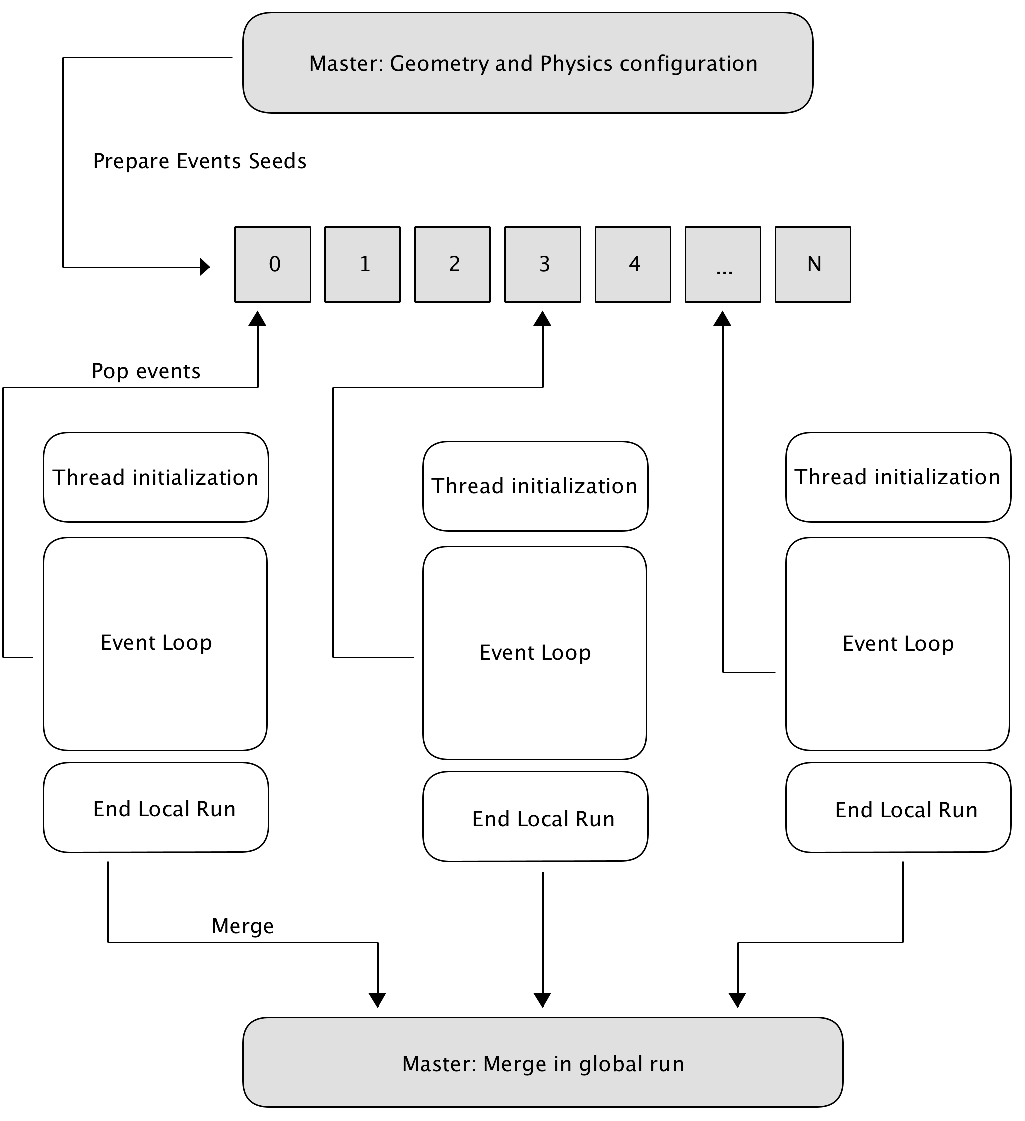
\includegraphics[width=0.47\textwidth]{figures/MTSchema.pdf}
\caption{Simplified description of a \Gfour{} multithreaded application: the
        {\it master} thread prepares geometry and physics setups for the simulation,
        and the {\it worker} threads compete for the next (group of) events to be
        simulated; otherwise they are independent.}
\label{fig:MTschema}
\end{figure}

\begin{figure}[htb]
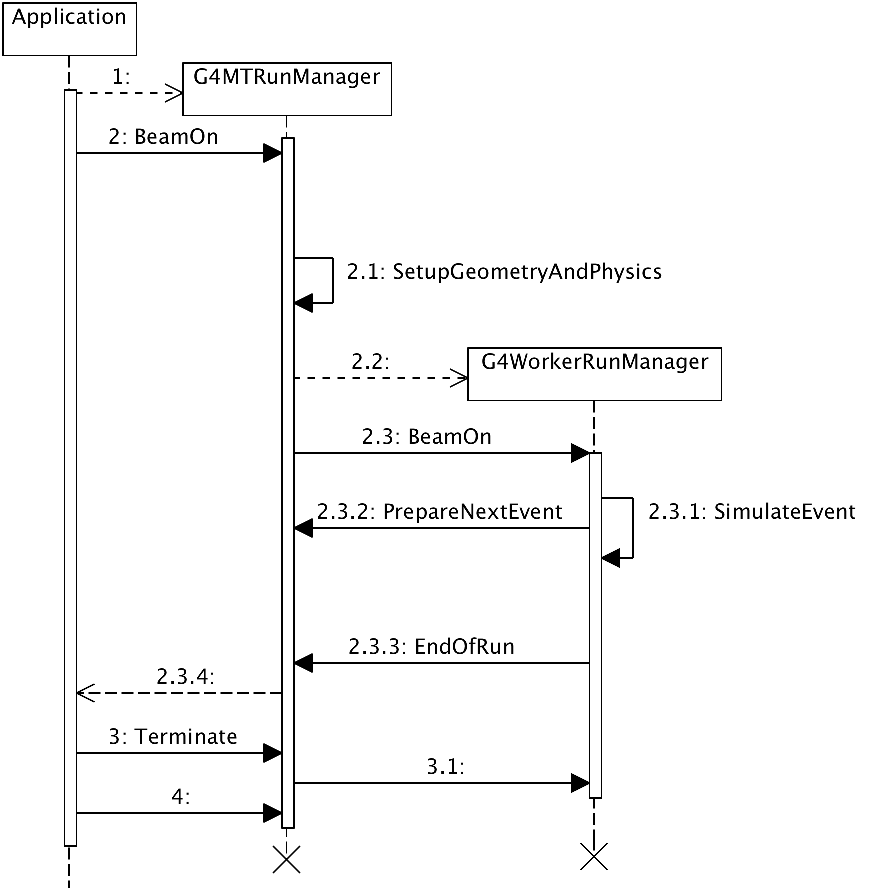
\includegraphics[width=0.45\textwidth]{figures/MTSimpleLife2A.pdf}
\caption{Sequence diagram of a multithreaded \Gfour{} application. The 
         application instantiates one \gclass{G4MTRunManager}.  When the 
         first run is started one or more worker threads are spawned. 
         The simulation in each worker thread is controlled by the local
         \gclass{G4WorkerRunManager}.}
\label{fig:MTlifecycle}
\end{figure}

\begin{figure}[htb]
    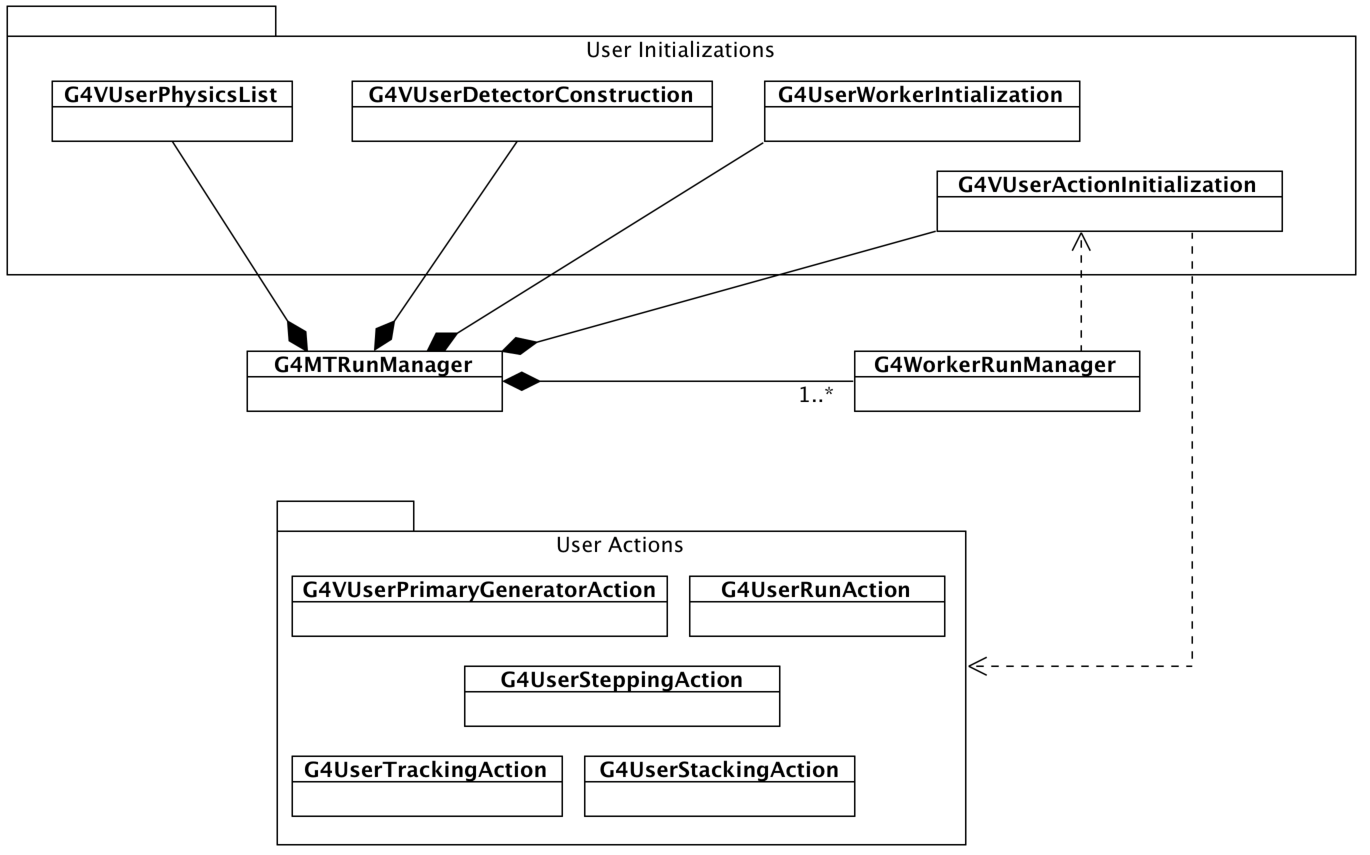
\includegraphics[width=0.45\textwidth]{figures/MTGeneralPaper2.pdf}
  \caption{Class diagram of the main user interfaces \cite{MT:TDG}. 
           User initializations (e.g. geometry and physics list) are shared
           among threads and are assigned to the single instance of
           \gclass{G4MTRunManager}, while user actions are created for each 
           thread (via \gclass{G4VUserActionInitialization}) and assigned to 
           the thread-private \gclass{G4WorkerRunManager}.}
  \label{fig:design}
\end{figure}

\subsection{\textbf{General Design}}
As a Monte Carlo simulation toolkit, \Gfour{} profits from improved throughput
via parallelism derived from the independence of modeled events and their 
computation.  Until \Gfour{} version 10.0, parallelization was obtained with a
simple distribution of inputs: each computation unit (e.g. a core of a node in a
cluster) ran a separate instance of \Gfour{} that was given a separate set of 
input events and associated random number seeds.

Given a computer with {\it k} cores, the design goal of multithreaded \Gfour{} was
to replace {\it k} independent instances of a \Gfour{} process with a single, 
equivalent process with {\it k} threads using the many-core machine in a 
memory-efficient, scalable manner.  The corresponding methodology involved 
transforming the code for thread safety and memory footprint reduction
\cite{MT:SNA2013}.  A simplified schema of the multithreading model used is 
shown in Figure~\ref{fig:MTschema}.  

Before the parallel section of the simulation begins, the geometry and physics
configurations are prepared and the random number engine is initialized in order
to generate a random sequence of uniformly distributed numbers.  This guarantees
reproducibility (see below).  Threads compete for the next group of events to be 
simulated, requesting one or more seeds from the shared seeds queue.  Output 
produced by the threads can be reduced at the end of the run.  If the application
uses the command-line scoring mechanism or histograms from the \Gfour{} analysis 
package, output from these is reduced automatically.  User-defined 
\gclass{G4Run} instances can be merged if they implement a \gmethod{Merge} method.

The multithreading option is based on a {\it master-worker} model in which one 
control sequence (the {\it master}) is responsible for initializing the geometry
and physics, and for spawning and controlling {\it worker} threads.  Workers are 
responsible for the simulation of one or more events.  The sequence diagram of a
\Gfour{} application is shown in Figure~\ref{fig:MTlifecycle} where the main 
interfaces (\gclass{G4MTRunManager} and \gclass{G4WorkerRunManager}) and their 
interactions are shown.

A \Gfour{} application is defined by the use of an instance of the 
\gclass{G4Run\allowbreak{}Manager} class or of a user-defined class derived from
it.  This class defines the main interaction with the user: it provides 
interfaces to define the {\it user initializations} (e.g. geometry and physics 
definitions) and the {\it user actions} that permit interaction with the 
simulation kernel and retrieve output information.  In particular,
\gclass{G4Run\allowbreak{}Manager} provides the interface to start the 
simulation of a run, which is a collection of events.  For multithreaded 
applications a derived class \gclass{G4MTRun\allowbreak{}Manager} is used 
that allows the number of worker threads to be specified.  Shared objects, such
as the geometry and physics list, are registered by the user to the instance of
this class, while the creation of user actions is the responsibility of a new 
class \gclass{G4VUserActionInitialization}.  When a new run is requested it is 
the responsibility of \gclass{G4MTRunManager} to start and configure worker 
threads.  Each thread owns an instance of \gclass{G4WorkerRunManager} and it 
shares only the user initialization classes, while it owns a private copy of the
user action classes.  Workers continue to request events from the master until 
there are no more events left in the current run.  At the end of the run the 
results collected by threads can be merged in the global run.

The communication between master and workers was implemented with a simple 
barrier mechanism to synchronize threads, and with the exchange of simple 
threading messages which currently may be one of:
\begin{itemize} 
\item {\it workers start new run} (instruct worker threads to begin the event
      loop),
\item {\it workers terminate} (instruct workers that the job has concluded, 
      workers should terminate and exit), or
\item {\it wait for workers ready} (master thread is waiting for one or more 
      workers to terminate current event loop, idle workers wait for further 
      messages).
\end{itemize}
User-defined code can be implemented by specializing key interfaces of certain
classes.  In particular, the \gclass{G4UserWorker\allowbreak{}Initialization} 
class defines the threading model and determines how threads are configured.  
The main \Gfour{} classes relevant to a multithreaded application are depicted
in Figure~\ref{fig:design}.  All interfaces are also available in sequential 
mode so that user code for a simulation application can be run both in 
multithreaded or sequential \Gfour{} with minimal changes.

\subsection{\textbf{Results}}
The physics and CPU performance of \Gfour{} were measured by comparing the
sequential version of the code to a multithreaded equivalent.  The results which
follow were obtained with a patched version of \Gfour{} Version 10.0, and 
%10.0.-ref0X
focus on high energy physics applications.  This domain was chosen because its 
complex physics requirements cover the most important use-cases for \Gfour{} 
users:
\begin{itemize}
\item high and low energy electromagnetic physics,
\item high and low energy hadronic physics, 
\item tracking in many-volume geometries and
\item tracking in electromagnetic fields.
\end{itemize}
In the near future regular testing will be extended to other user domains such
as medicine and space science.

So far, two applications have been adapted to multithreading.  The first is a 
test suite (Simplified Calorimeter) based on a simple geometry setup which allows
the study of all types of primary particle species over a very wide energy
range\cite{MT:6154433}.  The most interesting particles are electrons and hadrons
at high energy because they exercise the majority of physics models used in HEP
simulations of full showers.  Optional analyses can be performed on the 
predictions of the simulation in order to study typical HEP quantities.  These 
include both integral quantities like the total energy deposit, and detailed 
aspects of showers such as the number and type of interactions, and the energy 
spectra of produced secondaries.

The second application uses the \Gfour{} GDML interface\cite{MT:GDML} to
read a realistic geometry description of the CMS experiment at the LHC 
\cite{MT:collaboration2008cms}.  No analysis of simulated data is performed, but
a large set of materials and geometrical shapes is tested.  This application has
been used to test physics performance on different hardware setups, including 
Intel Xeon, ARM, PowerPC and Intel Atom processors, and Intel Xeon Phi 
co-processors.

% \begin{figure}[htb]
%     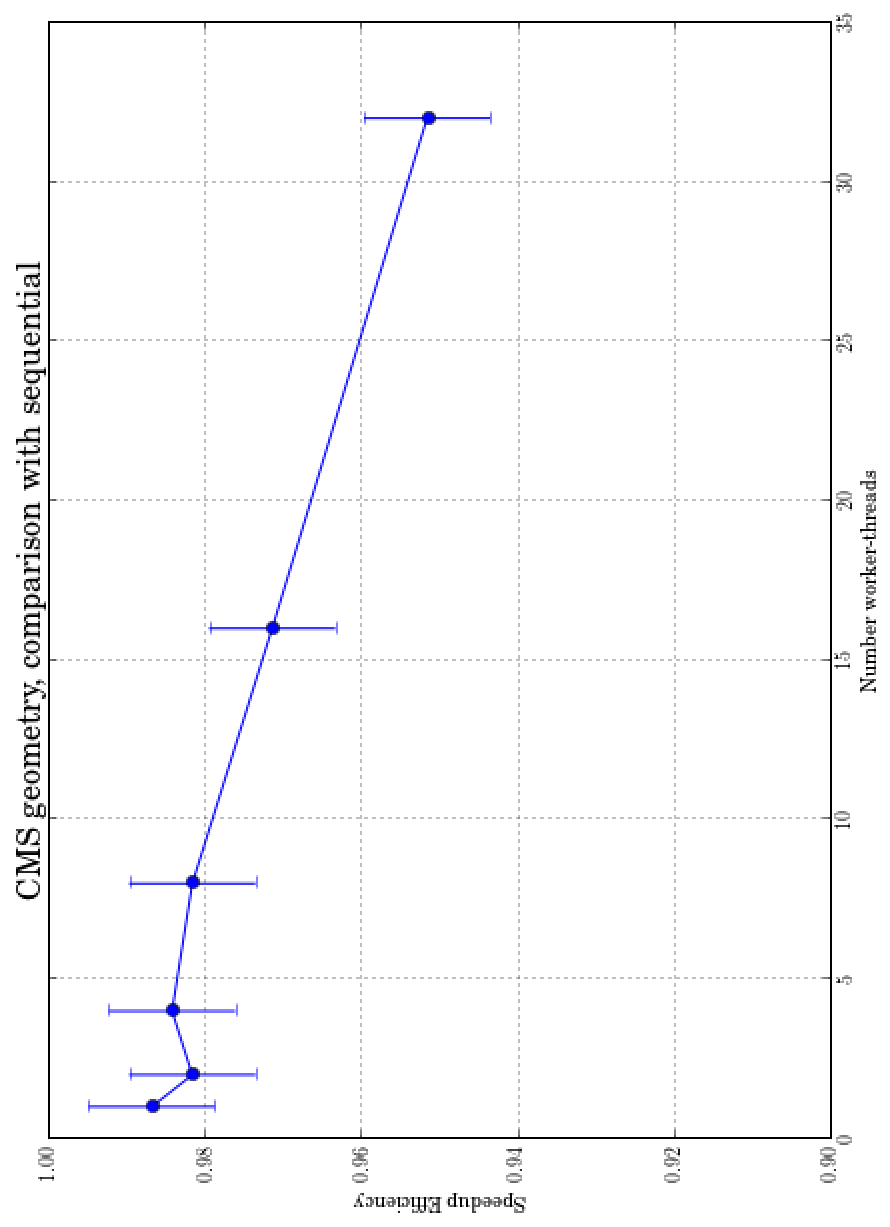
\includegraphics[width=0.35\textwidth, angle=-90]{figures/MTCPU.pdf}
%   \caption{Speedup efficiency (ratio of throughput of a run with {\it k} threads 
%            to the throughput of the sequential version), as a function of the 
%            number of threads, for the CMS simulation on an AMD-equipped server 
%            (Opteron Processor 6128 running at 2.40Hz, 4 CPU sockets x 8 cores). 
%            The multithreading overhead for one thread is only 1\%, while the 
%            efficiency is greater than 95\% for up to the maximum number of 
%            threads.} 
%   \label{fig:MTcpu}
% \end{figure}

\subsubsection{Physics equivalence to sequential}
It is of course required that the physics calculations are the same in both the
multithreaded and sequential versions.  Two tests were developed to verify this.
The first performs a statistical comparison of physics quantities simulated with
the Simplified Calorimeter testing suite.  Typical experimental observables 
(response, resolution and shower shapes) are compared between multithreaded
and sequential versions of the same application.  The resulting distributions 
were confirmed to be statistically equivalent. In this test the RNG engine seeds
used in the sequential and multithreading applications were not the same.

A more stringent test compares, event by event, the history of the random number
generator (RNG) engine.  To guarantee that reproducibility is independent of the 
number of threads and of the order in which events are simulated, each thread 
owns a separate instance of the RNG engine, and its status is re-initialized 
before the simulation of each event with a separate pre-defined seed.  The test
consists of two steps: a multithreaded application is run and the RNG engine 
seed recorded at the beginning of each event, together with the status of the 
engine at the end of the event simulation.  The same application is then run in
sequential mode, with the RNG engine re-initialized for each event with the seed
from the first run.  The engine status at the end of each event should be the 
same in the sequential and multithreaded versions.  It was verified that this 
occurs for 100\% of the cases, except for the test using the radioactive decay 
module.  This remaining discrepancy is being investigated, but it is thought to 
be due to violations of strict reproducibility - the independence of the 
results for a particular \Gfour{} event from the history of previous events.  
Extensive checking of the strong reproducibility of \Gfour{} physics models and 
physics lists has significantly reduced the incidence of such issues.  Strong
reproducibility of all classes used in a \Gfour{} application is an important 
requirement for providing consistent results in multithreaded runs, as results 
must not depend on the number of workers, or on the assignment of events to 
workers.
\begin{figure}[htb]
    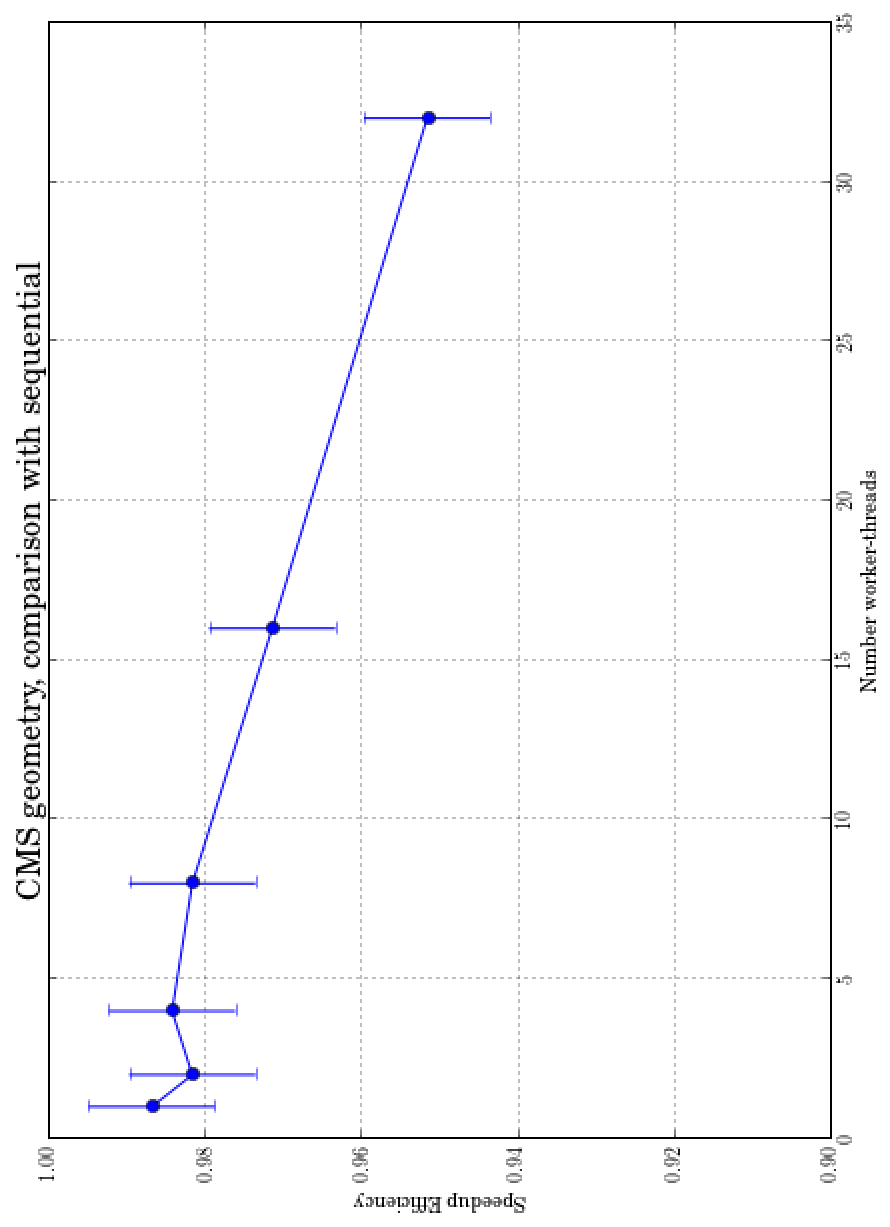
\includegraphics[width=0.35\textwidth, angle=-90]{figures/MTCPU.pdf}
  \caption{Speedup efficiency (ratio of throughput of a run with {\it k} threads
           to the throughput of the sequential version), as a function of the
           number of threads, for the CMS simulation on an AMD-equipped server
           (Opteron Processor 6128 running at 2.40Hz, 4 CPU sockets x 8 cores).
           The multithreading overhead for one thread is only 1\%, while the
           efficiency is greater than 95\% for up to the maximum number of
           threads.}
  \label{fig:MTcpu}
\end{figure}

\subsubsection{CPU and Memory performance}
The goal of event-level parallelism with threads is to reduce the memory 
footprint of parallel applications, while preserving the linear speedup of
throughput as a function of the number of physical cores.
Additional throughput is also expected in CPU architectures that support 
hyperthreading adding more workers~\cite{MT:leng2002study}.

Using the GDML geometry of the CMS application, three metrics were studied: the 
multithreading overhead with the number of threads {\it k} = 1 with respect to
a pure sequential application, the linearity of speedup as a function of the 
number of threads, and the memory reduction with respect to a multi-process 
approach.

In general, a performance penalty can be expected when comparing a sequential 
version of an application with the same version running with one worker thread.
In \Gfour{} this is due to the use of the \thread keyword that adds an additional 
indirection when accessing thread-private data. To remove this penalty a careful 
study of the use of \thread was carried out: compilation flags were chosen to 
minimize the impact of Thread Local Storage (TLS) selecting the best model for
\Gfour{} applications (\gkeyword{initial-exec}).  An overhead of ($\sim1$\%)
was measured as shown by the {\it k} = 1 point of Figure~\ref{fig:MTcpu}.

Figure~\ref{fig:MTcpu} shows the speedup linearity obtained with an AMD server
(Opteron Processor 6128 running at 2.0GHz, 4 CPU sockets x 8 cores) as a 
function of the number of threads, compared to the sequential case.  Good 
linearity was obtained with the CMS geometry simulation.  Speedup was linear 
with efficiencies of more than 95\%.  This result was confirmed on a number of 
different architectures: Intel Xeon, Intel Atom and PowerPC processors, ARM 
technology, and Intel Xeon Phi co-processors.  

Reported in Table~\ref{tab:MT:perf} is a comparison of the performance of 
different hardware executing the same CMS geometry application with the number
of threads equal to the number of logical cores.  Differences in performance 
were due mainly to the relative power of each core and the core multiplicity.  
The latest generation of Intel Xeon processor showed the best performance, 
expressed as absolute throughput (events/minute).

Figure~\ref{fig:memory} shows relative memory savings as a function of the
number of threads for the CMS geometry application.  \Gfour{} efficiently reduces
the memory used by the application when running with {\it k} threads 
({\it k}$>1$) compared to {\it k} copies of the same application.  For example, 
an application with eight threads requires about half the memory needed for 
eight clones of the sequential version of the same application.  The overhead 
with one worker thread is expected, since thread-private memory objects are
duplicated between worker and master threads.  The per-thread memory overhead
is at the level of 40--80~MB depending on the application (for the same 
application described in Table~\ref{tab:MT:perf} the sequential memory 
consumption is about 200~MB).
%  For a complex application like a HEP detector this is a good result.
 
\begin{table}[htdp]
\begin{center}
\begin{tabular}{|c|c|}
\hline
 & Throughput \\ Processor type & (events/min) \\
\hline
\hline
Intel Xeon X5650 - 2.67GHz & \\ 6 cores, x2 hyper-threaded & 320 \\
                                                 (with 12 sequential instances) & (324) \\\hline 
Intel Xeon E5-2695 v2 - 2.40GHz & \\12 cores, x2 hyper-threaded & 535 \\\hline
Intel Atom C2730 - 1.7GHz & \\ 8 cores & 74 \\ \hline
Exynos 5410 Octa Cortex-A15 & \\1.6GHz - 4 cores & 47 \\\hline
PowerPC A2 - 1.6GHz & \\ 16 cores, x4 hardware threads) & 119 \\\hline
Intel Xeon Phi 7120P - 1.238GHz & \\ 61 cores, x4 hyper-threaded & 334\\\hline
\end{tabular}
\end{center}
\caption{Comparison of different hardware when running CMS experiment geometry.
         Results show throughput (events/minute) per full processor.}
\label{tab:MT:perf}
\end{table}

% \begin{figure}[H]
\begin{figure}
    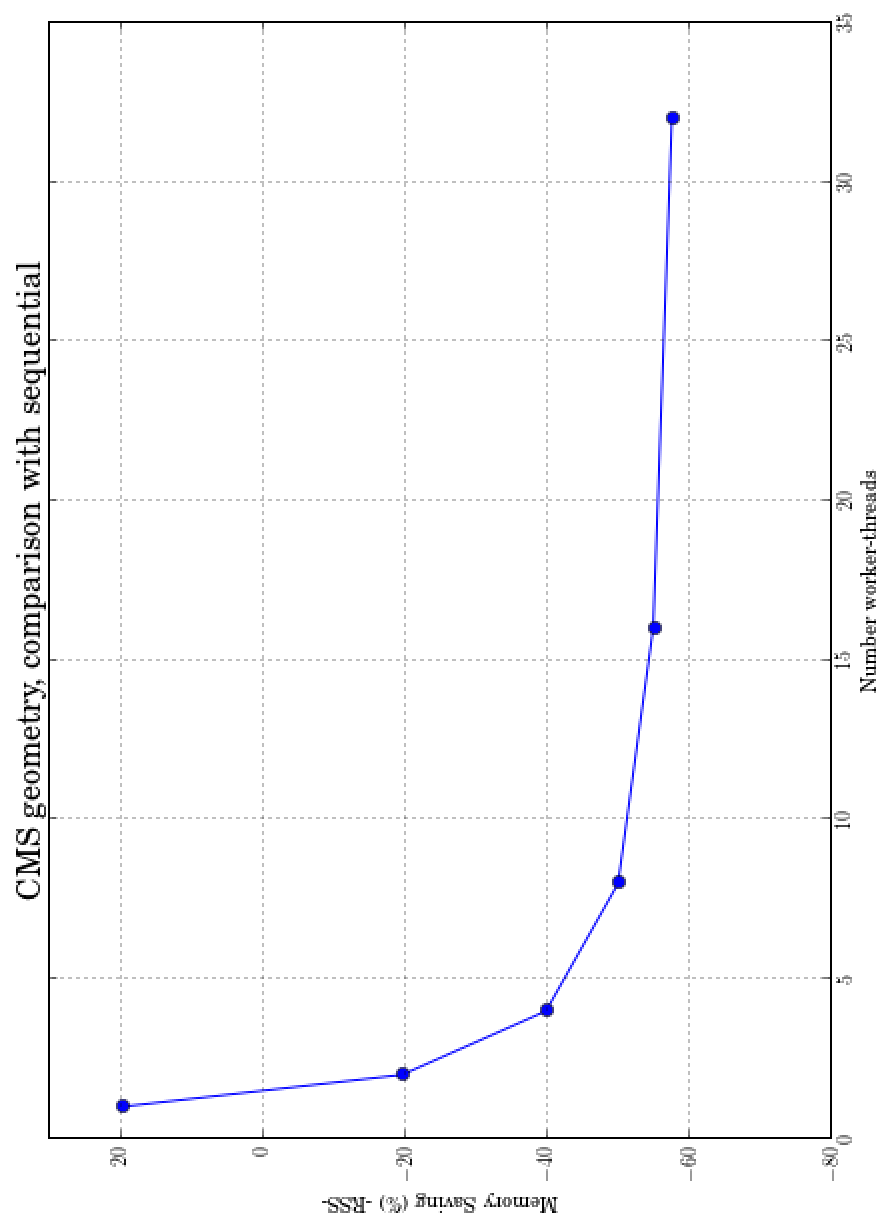
\includegraphics[width=0.35\textwidth, angle=-90]{figures/MTMEM.pdf}
  \caption{Relative memory reduction (memory used by a run with {\it k} 
           threads with respect to {\it k} instances of the sequential version),
           as a function of the number of threads, for the CMS simulation on an
           AMD equipped server (Opteron Processor 6128 running at 2.0GHz, 4 CPU
           sockets x 8 cores). The memory overhead with one worker thread is due 
           to the duplication of thread-private objects.  Already with two 
           worker threads, significant reduction of memory footprint is achieved.}
  \label{fig:memory}
\end{figure}

\subsection{\textbf{Further developments}}
Several improvements and extensions to the multithreading capabilities of 
\Gfour{} are planned for upcoming versions of the code.

With release 10.1 further reductions in the per-thread memory footprint of 
\Gfour{} applications are planned.  The most memory-consuming objects in typical 
simulations have been identified as hadronic cross sections, high precision
neutron models, reaction tables of the binary cascade models and the general 
particle source primary generator; strategies will be implemented to share these
objects among threads.  In some cases refinement of the design of the modules is
being carried out to better match the general multithreading strategy.  One goal
is to reduce the per-thread memory footprint by a factor of two.  This will 
allow applications to run on co-processors, where memory is of the order of GBs
and there are of order 100 threads.

Currently the number of threads is fixed and cannot be modified dynamically.
The planned removal of this restriction will achieve better integration with 
external parallelization frameworks such as Intel Threading Building Blocks 
(TBB)~\cite{MT:TBB}.  A prototype example,
\verb"examples/extended/parallel/TBB", that replaces \Gfour{}'s POSIX 
threading model with the TBB task-parallelism model, has already been released
with \Gfour{}, but improved and streamlined integration with this library is 
planned.

For several years now, \Gfour{} has provided an example, 
\verb"examples/extended/parallel/MPI", that demonstrates integration
with Message Passing Interface (MPI) \cite{MT:MPI}.  In version 10.0 this
example was migrated to a hybrid approach in which MPI ranks can exploit
multithreading to efficiently use memory-distributed systems.  Further 
refinement of the example is planned, with particular attention paid to 
providing merging of physics results.
